% Path of fire. The front-matter page from the 2024 draft (page v),
% placed here on a page of its own.
\thispagestyle{plain}
\begin{center}

\hspace{0pt}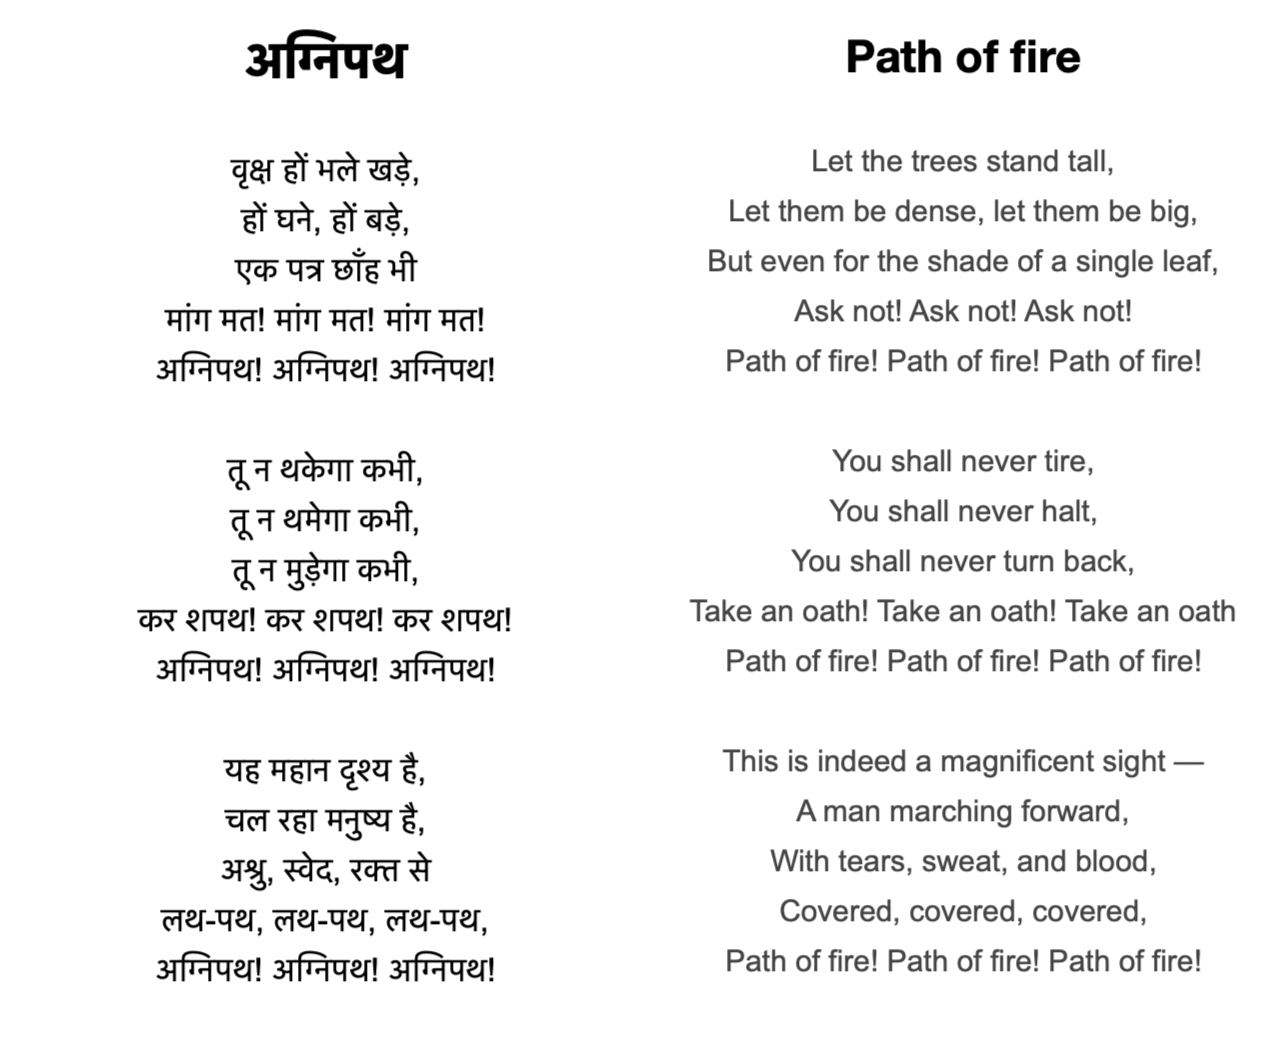
\includegraphics[width =0.74 \textwidth]{supplementary/figures/poemz.png}

A poem by Harivansh Rai Bachchan I've found interesting and have thought about a lot, especially in the final months, weeks and days of writing.\\


\vspace{12pt}
\noindent
Perhaps there is some implied causation from "not asking for shade" to the fact that the forest is thick and dense with trees. And in this regard,  there would be an analogy with the birth death catastrophe process: the propensity to "ask" aligning with catastrophe rate $\delta$, and large expected $\xt$ resulting from its diminishment -- the forest being dense and full of trees. \\

\vspace{12pt}
\noindent
When one pathway gets selected, the others in potential find themselves no-longer in the current basin of attraction. So without selection,  onward pathways can be numerous.  In the $\xt \to \infty$ limit, the draw from each diminishes to cessation.\\

\vspace{12pt}
\noindent
In a further (rather more dubious) potential analogy from here to the Vajrayana theory: the multifarious coloured lights of the bardo of dharmata \cite{trungpa2000tibetan} whizz and pop into a vast yet infinitely sub-divided tapestry,  without centre or circumference.  Leaving the journeyman undelivered,  thus unmarred, and increasingly without scope for reabsorption into the earthbound cycles of birth,  old age,  sickness and death. The essence of the teaching of the BT \cite{trungpa2000tibetan} seems,  as it were,  to "not ask" using means of being distracted by something else...

\end{center}
